% NOTE - this is only a template without real arguments
\begin{entry}{EdmCore and Callback Classes: step 1}{Aug 21, 2021}
    \objective 
    
    Get started on EDMCore. See if I can get a simulation running.

    \outline

    \begin{itemize}
        \item Retrieve useful code from the Log Test.
        \item Start filling in the methods.
        \item Add startup calls to the program's run routine.

    \end{itemize}

    \procedures
    
    Code them.

    \parameters
    
    N/A

    \observations
    
    Got it done. Everything worked smoothly. The MC is now able to initiate and run simulations from GridAPPS-D.
    It has the old issue where nothing stops, I'll have to hard code that in.
    Bigger issue: I started working with callback classes. The commands don't work. The sim runs, but nothing happens.
    The callbacks aren't called when expected. Need to talk to PNNL about this.

    \data
    
    All recorded data, or where it can be found.
    
    \results
    
    EDMCore is a bit more done than I was expecting, since I was able to do things like add config.txt.
    Callbacks are the next thing to tackle. I knew they'd be a problem, so this is fine. Consult with PNNL. Will report
    back in next entry.

\end{entry}


%\begin{entry}{CMake Error running EGOT-DCM Dockerfile}{Dec 02, 2020}
%    \objective
%
%    Determine the cause of the CMake error while running the dockerfile and modify file to get it to successfully build.
%
%    \outline
%
%    \begin{itemize}
%        \item Try running to see if it was just Lorry or a machine issue.
%        \item If it is a machine issue, modify configurations to ensure interoperability.
%        \item If I get the error track down its cause and modify dockerfile to fix.
%        \item Repeat until all builds are successful.
%    \end{itemize}
%
%    \procedures
%
%    \begin{itemize}
%        \item \mint{console}|git clone https://github.com/EGoT-DCS-SunSpec-Modbus|
%        \item \mint{console}|docker build -f Dockerfile.buster -t egot-dcs .|
%        \item \mint{console}|docker container run -i egot-dcs|
%    \end{itemize}
%
%    \observations
%
%    \begin{error}{Cmake Error: No CMAKE\_CXX\_COMPILER found}
%        \begin{figure}[H]
%            \centering
%            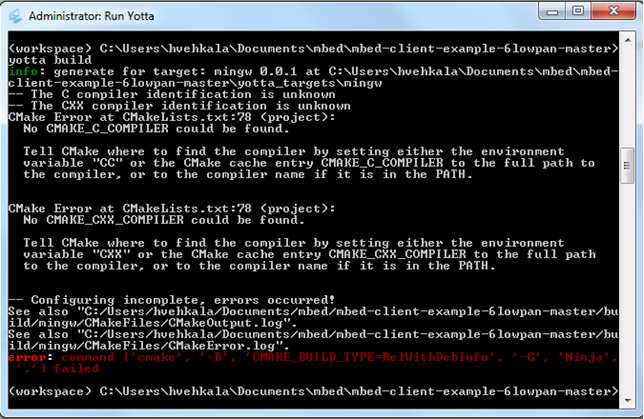
\includegraphics[height=4in]{Fall2020/Figures/cmake_error.png}
%        \end{figure}
%
%        Solution: what you need to do found at \cite{CMAKE-Forum}
%    \end{error}
%
%    \results
%
%    Short: No.
%
%    Long: Well...
%
%
%\end{entry}